\section{Method}

\subsection{Dataset}

There are several \gls{mri} and \gls{ct} datasets available, for
instance, \gls{oasis}~\cite{OASIS} or \gls{adni}~\cite{ADNI}. Unfortunately
public datasets in which both modalities are obtainable for the same subject
are, to date, rare. To our knowledge only the \gls{rire} project~\cite{RIRE}
and the Cancer Imaging Archive~\cite{CIA} provide \gls{mri} and \gls{ct}
volumes for some subjects. For the present work we limited ourselves to the
data from the \gls{rire} project, as the volumetric data was available in the
same format.
\begin{table}[h]
  \centering
  \begin{tabular}{*{6}{c}}
    \toprule
    & \multicolumn{4}{c}{\acrshort{mri}}
		& \\
   	\cmidrule{2-5}
    \acrshort{ct} &
		\acrshort{pd} &
		\acrshort{t1} &
		\acrshort{t2} &
		\acrshort{mp} \acrshort{rage} &
		\acrshort{pet} \\
    \midrule
    \num{17} & \num{14} & \num{19} & \num{18} & \num{9} & \num{8} \\
             & \num{12} & \num{17} & \num{16} & \num{9} & \num{6} \\
    \bottomrule
  \end{tabular}
  \caption{Subject statistics with respect of the available imaging
    modalities of the \gls{rire} dataset. The second table only accounts for
    subjects with available \gls{ct} data.
  }\label{tab:rire}
\end{table}
In \Cref{tab:rire} we list the aggregated modality count of the \gls{rire}
dataset (first row). As we use the \gls{ct} as target space, we created a
second modality count on the subjects with \gls{ct} modality (second row).
Beside of \gls{ct} one can also obtain \gls{pet} images for some subjects.
Next to the common \gls{t1} and \gls{t2} weighted \gls{mri}, some subjects of
the \gls{rire} dataset also offer \gls{pd} and \gls{mp} \gls{rage} weighted
\gls{mri}s. Some \gls{mri}s can be obtained in a rectified version, which we
did not use. We used the \gls{t1} weighted \gls{mri} together with the
\gls{ct} as input and target data as these give us the highest subject count.
However, it would be an interesting experiment to supply different \gls{mri}s
as multi-channel input.

\subsection{Preprocessing}

The modality data for each subject can be downloaded from the website of the
\gls{rire} project, see Ref.~\cite{RIRE}. In \Cref{fig:conversion} we depicted
the first preprocessing step, that involves the extraction, decompression and
conversion of the downloaded data. After extraction and decompression the
volumetric data presents itself as \gls{mhd}. We converted the \gls{mhd} files
to the self-contained \gls{nifti} format through the Python front-end of the
\gls{itk} library.
\begin{figure}[h]
  \centering
  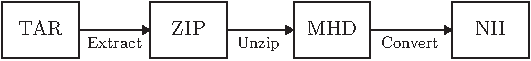
\includegraphics[width=\linewidth]{figure/conversion.pdf}
  \caption{Image extraction and conversion from \gls{mhd} to \gls{nifti}
		format.
	}\label{fig:conversion}
\end{figure}
\Cref{fig:registration} illustrates the coregistration procedure as part of
the image preprocessing. The coregistration yields a rigid transformation that
aligns the moving volume with the fixed volume. In our case it makes sense to
use the \gls{ct} volume as the fixed volume because the \gls{ct} are in
general better centered. Given a rigid transformation, a linear interpolator
returns a translated volume from the sample points of the initial \gls{mri}.
The mutual information between the moved \gls{mri} and the \gls{ct} is then
used to optimize the rigid transformation. The procedure is executed
iteratively and stopped when the maximum iterations steps are reached or
the convergence parameter is met. As the implementation of the interpolator
and transformation optimizer is not a trivial undergoing, therefore we
reverted back to the \gls{itk} library, see Ref.~\cite{Yaniv2018}.
\begin{figure}[h]
  \centering
  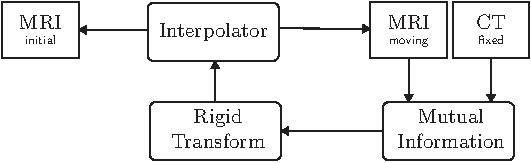
\includegraphics[width=\linewidth]{figure/registration.pdf}
  \caption{Multi-modal image coregistration using maximum mutual information
    optimizer.
	}\label{fig:registration}
\end{figure}
Finally we used a binary fill holes algorithm from SciPy~\cite{SciPy} to
remove the \gls{ct} table present in some \gls{ct} volumes as well as
background noise.\footnote{The complete preprocessing described so far is
available at \url{https://github/bodokaiser/mrtoct-scripts}.}

\subsection{Network}

As generative adversarial networks we decided to use pix2pix~\cite{Isola16}
as it has already shown great results in the task of color image to image
translation and context-aware 3d synthesis~\cite{Nie16} which uses a simpler
generator but accounts for 3d structures.

As convolutional encoder-decoder network we chose u-net~\cite{Ronneberger15}
as it was able to compete with much larger models in the task of semantic
segmentation~\cite{Badrinarayanan15}. Further our implementation of pix2pix
uses u-net as generator network, hence we are able to evaluate the impact
of the adversarial min-max approach.

\subsubsection{u-net}

\begin{figure}[h]
  \centering
  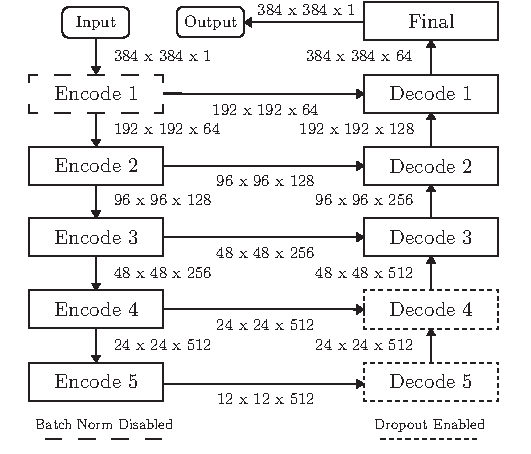
\includegraphics[width=\linewidth]{figure/unet-gen.pdf}
  \caption{The u-net generator architecture.
	}\label{fig:unet:gen}
\end{figure}
\begin{table}[h]
  \centering
  \begin{tabular}{lcccc}
    \toprule
    Block & Kernel & Strides & Padding & Initializer \\
    \midrule
    Encode & \num{4} & \num{2} & Same & Xavier \\
    Decode & \num{4} & \num{2} & Same & Xavier \\
    Final  & \num{3} & \num{2} & Same & Xavier \\
    \bottomrule
  \end{tabular}
  \caption{Convolution parameters used in the u-net blocks.
  }\label{tab:unet:conv}
\end{table}
\begin{figure}[h]
  \centering
  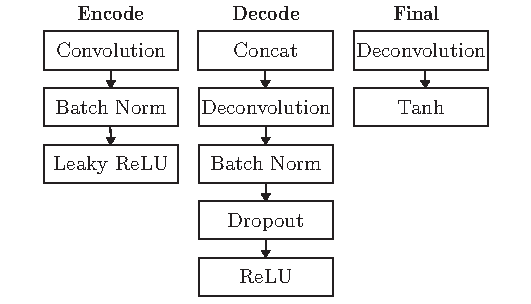
\includegraphics[width=\linewidth]{figure/unet-blocks.pdf}
  \caption{The u-net encoder, decoder and final convolution block.
	}\label{fig:unet:blocks}
\end{figure}

\subsubsection{pixtopix}

\begin{figure}[h]
  \centering
  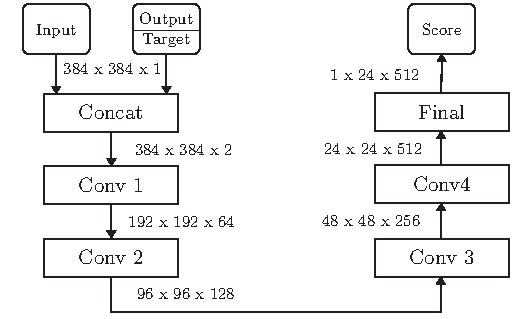
\includegraphics[width=\linewidth]{figure/pixtopix-disc.pdf}
  \caption{The pixtopix discriminator architecture.
	}\label{fig:pixtopix:disc}
\end{figure}
\begin{figure}[h]
  \centering
  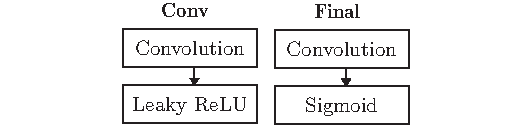
\includegraphics[width=\linewidth]{figure/pixtopix-blocks.pdf}
  \caption{The pixtopix discriminator blocks.
	}\label{fig:pixtopix:blocks}
\end{figure}

\subsubsection{3D Synthesis}

\begin{figure}[h]
  \centering
  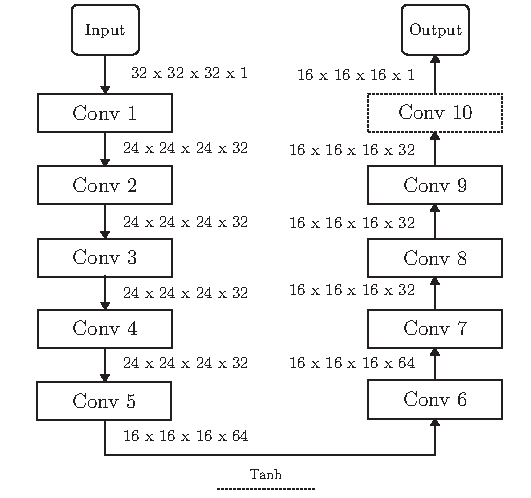
\includegraphics[width=\linewidth]{figure/synthesis-gen.pdf}
  \caption{The 3D synthesis generator architecture.
	}\label{fig:synthesis:gen}
\end{figure}
\begin{figure}[h]
  \centering
  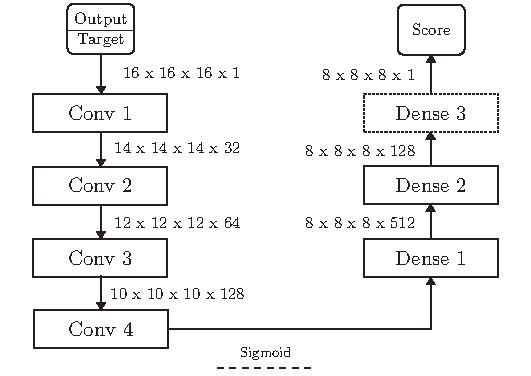
\includegraphics[width=\linewidth]{figure/synthesis-disc.pdf}
  \caption{The 3D synthesis discriminator architecture.
	}\label{fig:synthesis:disc}
\end{figure}
\begin{figure}[h]
  \centering
  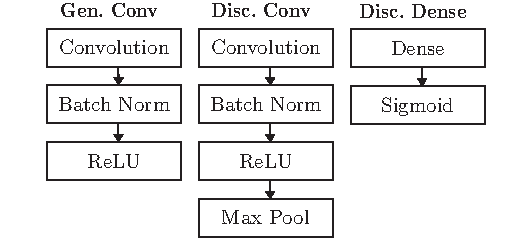
\includegraphics[width=\linewidth]{figure/synthesis-blocks.pdf}
  \caption{The 3D synthesis generator and discriminator dense and convolution
    blocks.
	}\label{fig:synthesis:blocks}
\end{figure}

\subsection{Losses}

\subsubsection{Distance Losses}

As norm losses we refer to the mean absolute error ($L1$ loss) and the
mean squared error ($L2$ loss).

\subsubsection{Gradient Losses}

The gradient (difference) loss is used in the framework of context-aware
3d synthesis~\cite{Nie16} in addition to the norm loss.

\subsubsection{Signal Losses}

From signal processing PSNR,SSE

\subsubsection{Adversarial Loss}

Least-squared adversarial loss, standard adversarial loss. BEGAN loss?


\subsection{Augmentation}

\subsubsection{Random Crop}
\subsubsection{Rotation}
\subsubsection{Contast Adjustment}

